% !TEX program = xelatex
% Build:  xelatex RouteResQ_Mini_Project_Report.tex  (run twice for the contents and cross-references)
\documentclass[12pt,a4paper]{report}

% ---- Formatting specification: A4, Times New Roman, 12/14/16 pt, 1.5 spacing, 2 cm margins ----
\usepackage[a4paper,margin=2cm]{geometry}
\usepackage{fontspec}
\setmainfont{Times New Roman}[
  Path=C:/Windows/Fonts/,
  UprightFont=times.ttf,
  BoldFont=timesbd.ttf,
  ItalicFont=timesi.ttf,
  BoldItalicFont=timesbi.ttf
]
\setmonofont{Courier New}
\usepackage{amsmath}
\usepackage{graphicx}
\usepackage{setspace}
\usepackage{titlesec}
\usepackage{fancyhdr}
\usepackage{booktabs}
\usepackage{tabularx}
\usepackage{longtable}
\usepackage{array}
\usepackage{enumitem}
\usepackage{caption}
\usepackage{float}
\usepackage{placeins}
\usepackage{needspace}
\usepackage{xcolor}
\usepackage{tikz}
\usetikzlibrary{arrows.meta,positioning,shapes.geometric,shapes.multipart,fit,calc}
\usepackage[hidelinks]{hyperref}
\usepackage{xurl}
\usepackage{eso-pic}

\definecolor{RouteCyan}{HTML}{2EA9C5}
\definecolor{RouteGreen}{HTML}{3FAF83}
\definecolor{RouteAmber}{HTML}{C79A48}
\definecolor{RouteClay}{HTML}{C76555}
\definecolor{RouteBlue}{HTML}{688DD8}
\definecolor{RouteInk}{HTML}{1E2833}
\definecolor{RoutePale}{HTML}{EEF4F6}

\setstretch{1.5}
\setlength{\headheight}{14.5pt}
\setlength{\parindent}{0.45in}
\setlength{\parskip}{0.15em}
\setlength{\emergencystretch}{2em}
\setlist{itemsep=0.2em,topsep=0.25em,leftmargin=1.5em}
% Figure captions below figures, table titles above tables
\captionsetup{font=normalsize,labelfont=bf,justification=centering,skip=4pt}
\captionsetup[table]{position=top}
\setlength{\textfloatsep}{9pt plus 2pt minus 2pt}
\setlength{\floatsep}{8pt plus 2pt minus 2pt}
\setlength{\intextsep}{8pt plus 2pt minus 2pt}
\numberwithin{equation}{chapter}

% Chapter titles: "Chapter N: Title", 16 pt; sections 14 pt; subsections 12 pt
\titleformat{\chapter}[block]
  {\normalfont\bfseries\centering\fontsize{16}{19}\selectfont}
  {\chaptername\ \thechapter:}{0.35em}{}
\titleformat{name=\chapter,numberless}[block]
  {\normalfont\bfseries\centering\fontsize{16}{19}\selectfont}{}{0pt}{}
\titlespacing*{\chapter}{0pt}{-22pt}{16pt}
\titleformat{\section}{\normalfont\bfseries\fontsize{14}{17}\selectfont}{\thesection}{0.6em}{}
\titleformat{\subsection}{\normalfont\bfseries\fontsize{12}{15}\selectfont}{\thesubsection}{0.5em}{}

% Page numbers bottom-centre on every page (Roman for prelims, Arabic for chapters)
\pagestyle{fancy}
\fancyhf{}
\fancyhead[L]{\small RouteResQ Mini Project Report}
\fancyhead[R]{\small Computer Networks 24B15CS313}
\fancyfoot[C]{\thepage}
\renewcommand{\headrulewidth}{0.3pt}
\renewcommand{\footrulewidth}{0pt}
\fancypagestyle{plain}{\fancyhf{}\fancyfoot[C]{\thepage}\renewcommand{\headrulewidth}{0pt}}

\newcommand{\asset}[1]{routeresq_assets/#1}
\newcommand{\tighttable}{\renewcommand{\arraystretch}{1.18}}

\begin{document}

% Consistent page border throughout the report
\AddToShipoutPictureBG{%
  \AtPageLowerLeft{\put(34,34){\framebox(527,774){}}}%
}

% -----------------------------------------------------------------------------
% Title page
% -----------------------------------------------------------------------------
\begin{titlepage}
\thispagestyle{empty}
\begin{center}
\vspace*{0.12in}
{\large\bfseries Jaypee Institute of Information Technology, Noida\par}
\vspace{0.22in}
{\normalsize DEPARTMENT OF COMPUTER SCIENCE \& ENGINEERING AND\par}
{\normalsize INFORMATION TECHNOLOGY\par}

\vspace{0.38in}
{\large\bfseries Project Title: RouteResQ\par}
\vspace{0.08in}
{\large\bfseries Network Failure Detection, Routing Analysis\par}
{\large\bfseries and Secure Communication\par}

\vspace{0.38in}
\includegraphics[height=1.50in]{\asset{jiit-logo.png}}

\vspace{0.34in}
{\normalsize\bfseries Submitted By\par}
\vspace{0.14in}
\begingroup
\renewcommand{\arraystretch}{1.18}
\begin{tabular}{@{}>{\bfseries}r l >{\bfseries}r l@{}}
Enrolment No.: & 2408030010 & Name: & Saanvi Grover\\
Enrolment No.: & 2408030019 & Name: & Aditya Sharma\\
Enrolment No.: & 2408030011 & Name: & Prankit Goel\\
Enrolment No.: & 2408030026 & Name: & Aaradhya Shankar Kulashri
\end{tabular}
\endgroup

\vspace{0.20in}
{\normalsize\bfseries Submitted To\par}
\vspace{0.08in}
Dr. Kirti Aggarwal\hspace{0.70in}Dr. Kapil Madan

\vfill
\begingroup
\renewcommand{\arraystretch}{1.15}
\begin{tabular}{rl}
\textbf{Course Name:} & Computer Networks\\
\textbf{Course Code:} & 24B15CS313\\
\textbf{Program:} & B. Tech. CSE/IT\\
\textbf{Semester:} & Third Year, 5th Semester
\end{tabular}
\endgroup
\vspace{0.05in}
\end{center}
\end{titlepage}

% -----------------------------------------------------------------------------
% Preliminary pages (Roman numbering)
% -----------------------------------------------------------------------------
\pagenumbering{roman}
\setcounter{page}{1}

\chapter*{Abstract}
\addcontentsline{toc}{chapter}{Abstract}
RouteResQ is an integrated Computer Networks laboratory platform whose central goal is to identify the cause of a network failure, measure what the failure did to traffic, and observe whether and how service recovered. The completed system combines live diagnostics, a deterministic root-cause rule engine, four NS2 2.35 experiments, TCP and UDP socket communication, TLS certificate validation, SHA-256 integrity checking, controlled failure drills, a root-cause register, and generated reports in one Streamlit application, deployed publicly at \url{https://routeresq.streamlit.app}. Live measurements, simulations, and loopback socket experiments are deliberately kept separate so that a simulated cause is never presented as the cause of a live problem.

The live diagnostics module executes allow-listed DNS, gateway, ping, traceroute or tracert, and optional TCP-connect checks. Seventeen deterministic rules convert the measurements into findings, keep contradictory evidence visible, and label every conclusion as confirmed, likely, possible, or insufficient evidence. The root-cause register then gives every detected failure one cause status: \emph{Confirmed (injected)}, \emph{Likely}, \emph{Not confirmed}, or \emph{No failure detected}. The NS2 module analyses a six-node topology under a healthy baseline, a distance-vector link failure, a static-routing link failure, and congestion. Real NS2 traces show that distance-vector routing moved traffic to the alternative path with only two packet losses and a first alternative delivery 43.6 ms after the failure, whereas static routing produced a 3.024 s delivery gap and 37.66\% overall loss. Congestion filled a 20-packet DropTail queue and raised delay and loss until the competing flow stopped.

The communication module demonstrates framed TCP, sequenced UDP, TLS 1.3, certificate and host-name validation, and payload integrity. Six controlled drills cover refusal, timeout, reset, missing datagrams, an untrusted certificate, and a host-name mismatch, each followed by an explicit restoration check. A guided demonstration runs the whole Detect, Diagnose, Analyse impact, Observe recovery and Report sequence and verifies each stage against stored evidence. A suite of 159 automated tests validates the parsers, rules, simulations, sockets and user interface.

\textbf{Keywords:} network diagnostics, root-cause analysis, NS2, distance-vector routing, TCP, UDP, TLS, SHA-256, Streamlit.

\clearpage
\setcounter{tocdepth}{1}
\tableofcontents

\clearpage
\listoffigures
\addcontentsline{toc}{chapter}{List of Figures}

\clearpage
\listoftables
\addcontentsline{toc}{chapter}{List of Tables}

\clearpage
\pagenumbering{arabic}
\setcounter{page}{1}

% =============================================================================
\chapter{Introduction}
% =============================================================================

\section{Background}
Modern applications depend on several network layers working together. The same visible symptom, such as a timeout, may arise from a DNS failure, an unreachable destination, packet loss, congestion, a closed service port, or an application fault. In current practice a student or administrator runs \texttt{ping}, \texttt{traceroute}/\texttt{tracert} and \texttt{nslookup} one after another and interprets the raw output by hand. Each tool exposes only part of the path: routers may ignore ICMP, four echo requests give only coarse loss resolution, and a successful TCP connection can contradict a failed ping. Routing behaviour and recovery are usually studied separately in a simulator such as NS2 \cite{ns2book}, and socket programming and TLS \cite{tcp,udp,tls13} in yet another exercise.

RouteResQ brings these three environments together. Live diagnostics collect real operating-system measurements; NS2 2.35 injects known faults into a six-node topology so that routing impact and recovery can be measured from the simulator's own trace; and real socket experiments compare TCP, UDP, TLS identity validation, and SHA-256 integrity \cite{sha}. Independent Python modules and a Streamlit console \cite{streamlit} connect these environments while ensuring that every displayed claim comes from stored backend evidence.

\section{Problem Statement}
When a network service fails, the operational questions are: \emph{what failed, why did it fail, what happened to the traffic, did the service recover, and how certain is each answer?} Existing laboratory exercises answer these questions in isolation, and diagnostic tools report symptoms rather than causes. A user therefore either guesses one cause or cannot connect the measurement to the mechanism, and confident-sounding conclusions are often unsupported by the evidence. This matters both for teaching, where students learn to over-claim, and for operations, where a wrong cause wastes repair effort.

RouteResQ addresses this gap. Its objectives are to:
\begin{itemize}
  \item run authorised DNS, gateway, ping, path and TCP checks and classify the symptoms with traceable, deterministic rules;
  \item state the root cause of every detected failure together with an explicit certainty status rather than an invented confidence percentage;
  \item compare healthy, link-failure and congestion scenarios in NS2 and reconstruct packet paths, delay, throughput, loss, queues and recovery;
  \item compare real TCP and UDP behaviour, validate TLS certificates, host names and SHA-256 integrity, and demonstrate controlled transport failures with restoration; and
  \item export reports that remain linked to their JSON, CSV, Markdown and trace evidence.
\end{itemize}

\section{Social and Environmental Relevance}
RouteResQ turns commands and packet events into an auditable explanation of a failure. This reduces trial-and-error troubleshooting, shortens the time needed to isolate a fault, and teaches precise language about what a measurement can and cannot prove. Because the experiments run on ordinary computers and in a simulator, a whole class can study routing failure, congestion and secure transport without dedicated routers, switches or traffic generators, which lowers equipment cost, energy use and electronic waste. Active probing is restricted to authorised destinations, so the tool cannot be turned against third-party networks.

\textbf{Primary SDG(s):} SDG 9 -- Industry, Innovation and Infrastructure. The project contributes to resilient network infrastructure by explaining how routing reacts to link failure, how congestion degrades service, and how secure, integrity-checked communication is verified.

\textbf{Secondary SDGs:} SDG 4 -- Quality Education, through repeatable, evidence-driven experiments for Computer Networks students; and SDG 12 -- Responsible Consumption and Production, by reusing existing computers and simulation instead of additional networking hardware.

\section{Scope}
The project covers:
\begin{itemize}
  \item live DNS, gateway, ping, traceroute/tracert and TCP-connect diagnostics against loopback, private or explicitly authorised destinations, on Windows and Linux;
  \item a deterministic root-cause engine with baselines, route comparison, rule traces and a cross-source root-cause register;
  \item four NS2 2.35 scenarios with packet-level trace analysis, phase metrics and recovery observation;
  \item TCP and UDP sockets, TLS 1.2+ with a local lab PKI, SHA-256 integrity and six controlled failure drills; and
  \item a Streamlit interface with a guided demonstration, Markdown reports and evidence export.
\end{itemize}
Its boundaries are equally explicit. RouteResQ does not capture packets, detect intrusions, use machine learning, repair live networks automatically, manage enterprise devices, or implement custom cryptography. NS2 results describe the configured model rather than any real network, and loopback measurements exclude realistic propagation delay and path loss. The public deployment further restricts probing to well-known public destinations.

% =============================================================================
\chapter{System Design \& Methodology}
% =============================================================================

\section{Proposed Methodology}
RouteResQ follows a five-stage, evidence-first methodology: \textbf{Detect} (collect measurements), \textbf{Diagnose} (apply deterministic rules and state a cause with its certainty), \textbf{Analyse impact} (quantify what the failure did to traffic), \textbf{Observe recovery} (claim recovery only when evidence shows it), and \textbf{Report} (store and export every artefact). Each stage writes its evidence to disk before the next stage reads it, so every conclusion in the interface or in a report can be traced back to a measurement, a trace event, or a deliberately injected condition. The same five stages form the navigation rail of the Streamlit application and the steps of its guided demonstration. The following subsections describe the architecture, the workflow, the object-oriented design, and the method used in each evidence environment.

\subsection{System Architecture}
The implementation separates presentation, measurement, analysis and storage, as summarised in Figure~\ref{fig:architecture}. Streamlit pages call Python modules but contain no networking logic, so the same diagnostics, simulation analysis, socket experiments and report generation can be used from the command line and from the test suite. The principal backend packages are \texttt{diagnostics}, \texttt{failure\_analysis}, \texttt{simulation}, \texttt{analysis}, \texttt{communication}, \texttt{security} and \texttt{walkthrough}; the \texttt{app\_pages} and \texttt{ui} layers only present stored evidence.

\begin{figure}[htbp]
\centering
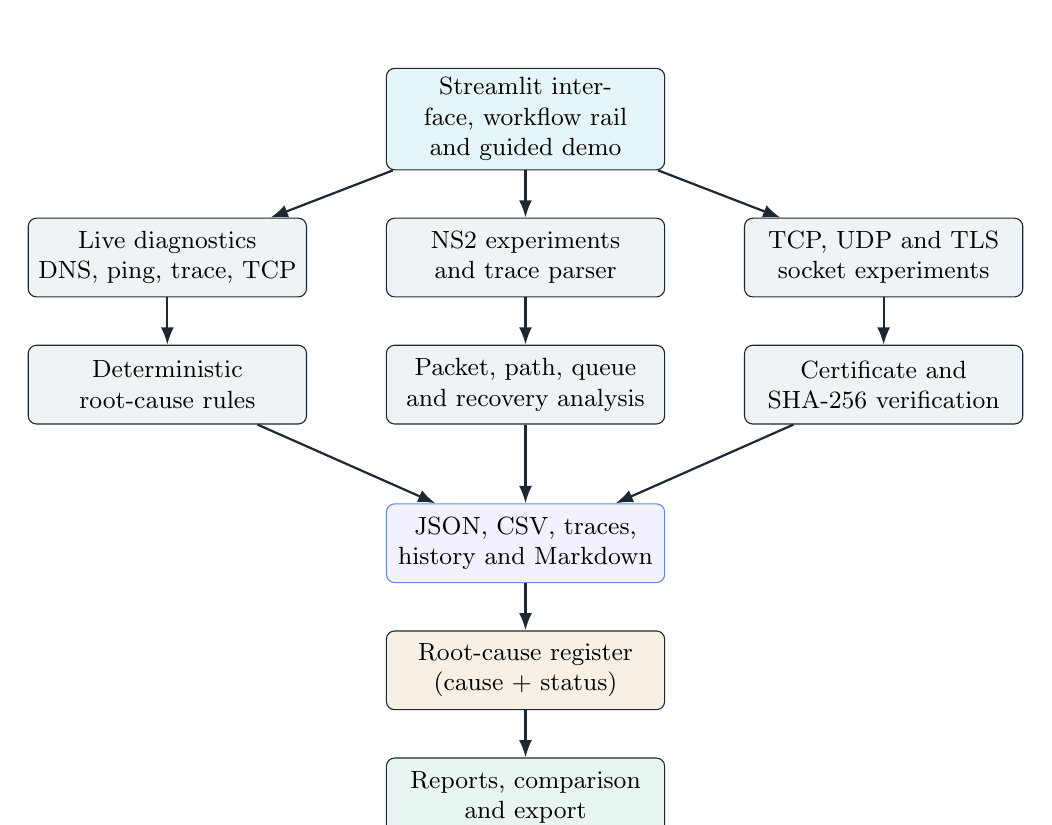
\begin{tikzpicture}[
  node distance=6mm and 10mm,
  box/.style={draw=RouteInk,rounded corners=3pt,align=center,minimum height=10mm,text width=33mm,fill=RoutePale,font=\small},
  data/.style={draw=RouteBlue,rounded corners=3pt,align=center,minimum height=10mm,text width=33mm,fill=blue!5,font=\small},
  arrow/.style={-{Latex[length=2.2mm]},thick,draw=RouteInk}
]
\node[box,fill=RouteCyan!12] (ui) {Streamlit interface, workflow rail and guided demo};
\node[box,below left=of ui] (diag) {Live diagnostics\\DNS, ping, trace, TCP};
\node[box,below=of ui] (sim) {NS2 experiments\\and trace parser};
\node[box,below right=of ui] (comm) {TCP, UDP and TLS\\socket experiments};
\node[box,below=of diag] (rules) {Deterministic\\root-cause rules};
\node[box,below=of sim] (analysis) {Packet, path, queue\\and recovery analysis};
\node[box,below=of comm] (security) {Certificate and\\SHA-256 verification};
\node[data,below=10mm of analysis] (store) {JSON, CSV, traces,\\history and Markdown};
\node[box,below=of store,fill=RouteAmber!15] (register) {Root-cause register\\(cause + status)};
\node[box,below=of register,fill=RouteGreen!12] (report) {Reports, comparison\\and export};
\draw[arrow] (ui) -- (diag);
\draw[arrow] (ui) -- (sim);
\draw[arrow] (ui) -- (comm);
\draw[arrow] (diag) -- (rules);
\draw[arrow] (sim) -- (analysis);
\draw[arrow] (comm) -- (security);
\draw[arrow] (rules) -- (store);
\draw[arrow] (analysis) -- (store);
\draw[arrow] (security) -- (store);
\draw[arrow] (store) -- (register);
\draw[arrow] (register) -- (report);
\end{tikzpicture}
\caption{RouteResQ system architecture}
\label{fig:architecture}
\end{figure}

\subsection{Overall Workflow}
The user begins with a live diagnostic or a stored experiment. RouteResQ validates the requested destination or scenario before any command runs, normalises the measurements into a common evidence model, and passes them to the live rule engine or to the simulation and transport analysers. The flowchart in Figure~\ref{fig:workflow} shows the complete sequence, including the branch on the evidence environment that keeps live, simulated and loopback results apart.

\begin{figure}[htbp]
\centering
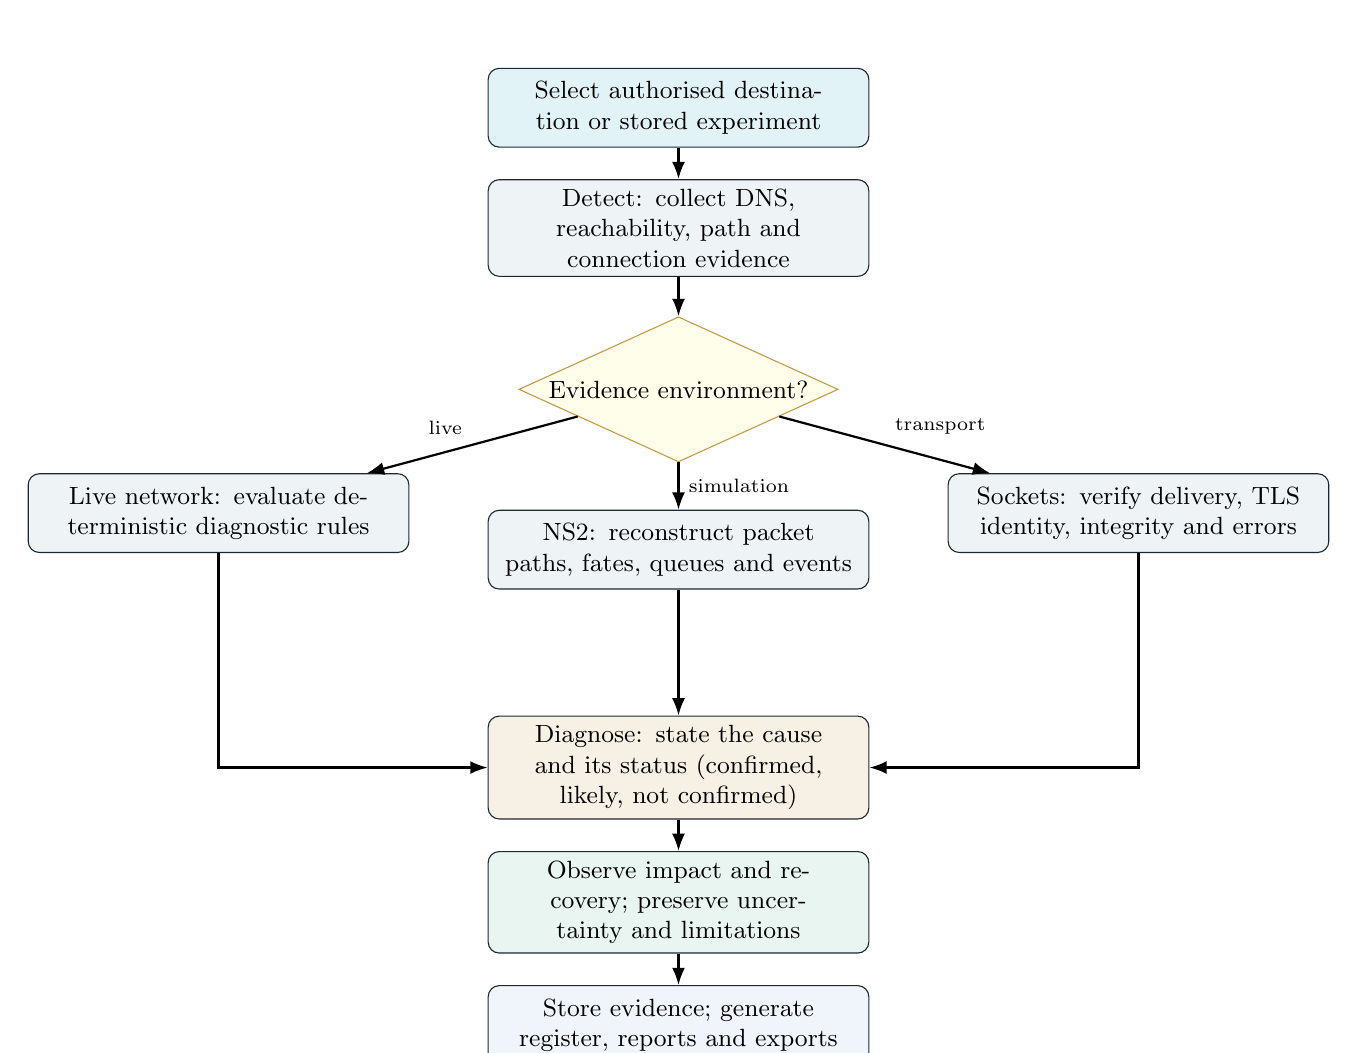
\begin{tikzpicture}[
  node distance=4mm,
  stage/.style={draw=RouteInk,rounded corners=4pt,align=center,text width=46mm,minimum height=10mm,fill=RoutePale,font=\small},
  decision/.style={diamond,draw=RouteAmber,aspect=2.2,align=center,fill=yellow!8,font=\small,inner sep=1.2pt},
  arrow/.style={-{Latex[length=2.2mm]},thick}
]
\node[stage,fill=RouteCyan!14] (start) {Select authorised destination or stored experiment};
\node[stage,below=of start] (detect) {Detect: collect DNS, reachability, path and connection evidence};
\node[decision,below=5mm of detect] (kind) {Evidence environment?};
\node[stage,below left=6mm and 24mm of kind] (live) {Live network: evaluate deterministic diagnostic rules};
\node[stage,below=6mm of kind] (ns2) {NS2: reconstruct packet paths, fates, queues and events};
\node[stage,below right=6mm and 24mm of kind] (sock) {Sockets: verify delivery, TLS identity, integrity and errors};
\node[stage,below=16mm of ns2,fill=RouteAmber!15] (cause) {Diagnose: state the cause and its status (confirmed, likely, not confirmed)};
\node[stage,below=of cause,fill=RouteGreen!12] (recovery) {Observe impact and recovery; preserve uncertainty and limitations};
\node[stage,below=of recovery,fill=RouteBlue!10] (report) {Store evidence; generate register, reports and exports};
\draw[arrow] (start) -- (detect);
\draw[arrow] (detect) -- (kind);
\draw[arrow] (kind) -- node[above left,font=\scriptsize]{live} (live);
\draw[arrow] (kind) -- node[right,font=\scriptsize]{simulation} (ns2);
\draw[arrow] (kind) -- node[above right,font=\scriptsize]{transport} (sock);
\draw[arrow] (live) |- (cause);
\draw[arrow] (ns2) -- (cause);
\draw[arrow] (sock) |- (cause);
\draw[arrow] (cause) -- (recovery);
\draw[arrow] (recovery) -- (report);
\end{tikzpicture}
\caption{Flowchart of the evidence-driven RouteResQ workflow}
\label{fig:workflow}
\end{figure}

\subsection{Object-Oriented Design}
The backend is modelled as small classes with one responsibility each. Figure~\ref{fig:uml} is a UML class diagram of the principal classes. Measurement results are immutable-style data classes composed into a \texttt{DiagnosticRun}; the rule engine turns a run into an \texttt{AnalysisReport}; an NS2 \texttt{Scenario} is executed by an \texttt{NS2Backend} into a \texttt{SimulationRun} whose trace is reconstructed into \texttt{PacketRecord} objects; and the transport layer is built from a reusable \texttt{TCPTransferServer}, a \texttt{TransferResult} returned by the client, and a \texttt{LabPKI} used by the TLS demonstration. Command execution is abstracted behind the \texttt{CommandRunner} protocol, so the tests substitute a fake runner that replays captured Windows and Linux output.

\begin{figure}[htbp]
\centering
\begin{tikzpicture}[
  font=\scriptsize,
  cls/.style={rectangle split,rectangle split parts=3,draw=RouteInk,text width=44mm,
              rectangle split part align={center,left,left},
              rectangle split part fill={RouteCyan!14,white,white},inner sep=2pt},
  node distance=7mm,
  real/.style={-{Triangle[open,length=2.4mm]},dashed,thick},
  dep/.style={-{Stealth[length=2.2mm]},dashed},
  comp/.style={{Diamond[length=2.6mm,width=1.8mm]}-,thick},
  lbl/.style={font=\tiny,fill=white,inner sep=1pt}
]
% ---- diagnostics / failure_analysis ----
\node[cls] (runner) at (0,0) {\textit{\guillemotleft protocol\guillemotright}\\\textbf{CommandRunner}
  \nodepart{two} \vphantom{x}
  \nodepart{three} + run(argv, timeout)\\\hspace*{1em}: CommandRecord\\+ available(exe): bool};
\node[cls,below=of runner] (sub) {\textbf{SubprocessRunner}
  \nodepart{two} allow-listed executables
  \nodepart{three} + run(argv, timeout)\\+ available(exe)};
\node[cls,below=of sub] (run) {\textbf{DiagnosticRun}
  \nodepart{two} run\_id, target, timestamp\\dns: DNSResult; ping: PingResult\\traceroute: TracerouteResult\\tcp\_check: TCPCheckResult
  \nodepart{three} + to\_dict()};
\node[cls,below=10mm of run] (rep) {\textbf{AnalysisReport}
  \nodepart{two} classifications, conclusion\\findings: list[Finding]\\explanations: list[Explanation]\\rule\_trace: list[RuleTrace]
  \nodepart{three} + to\_dict()};
% ---- simulation / analysis ----
\node[cls] (scn) at (5.65,0) {\textbf{Scenario}
  \nodepart{two} id, category, known\_cause\\params, phases, flows: Flow
  \nodepart{three} + \_\_post\_init\_\_(): validate};
\node[cls,below=of scn] (be) {\textbf{NS2Backend}
  \nodepart{two} kind: local | docker\\version
  \nodepart{three} run\_scenario(scenario)};
\node[cls,below=of be] (sr) {\textbf{SimulationRun}
  \nodepart{two} scenario\_id, trace\_file\\events\_file, ns\_version
  \nodepart{three} load\_run(dir)};
\node[cls,below=10mm of sr] (pkt) {\textbf{PacketRecord}
  \nodepart{two} pkt\_id, send\_time, recv\_time\\hops, drop, fate
  \nodepart{three} build\_packet\_records(trace)};
% ---- communication / security ----
\node[cls] (srv) at (11.3,0) {\textbf{TCPTransferServer}
  \nodepart{two} host, port, ssl\_context\\abort\_after\_bytes, events
  \nodepart{three} + start()  + stop()\\+ \_\_enter\_\_()  + \_\_exit\_\_()};
\node[cls,below=of srv] (tr) {\textbf{TransferResult}
  \nodepart{two} ok, tls, bytes\_sent\\throughput\_mbps, integrity\_ok
  \nodepart{three} classify\_error(exc)};
\node[cls,below=of tr] (pki) {\textbf{LabPKI}
  \nodepart{two} ca\_cert, server\_cert\\rogue\_ca\_cert, wrong\_host\_cert
  \nodepart{three} ensure\_lab\_pki()};
\node[cls,below=10mm of pki] (fr) {\textbf{FailureRecord}
  \nodepart{two} failure\_type, condition\_created\\observed\_error, resumed
  \nodepart{three} demo\_*() drills};
% ---- cause register (utility module) ----
\node[cls,text width=60mm,below=12mm of pkt,rectangle split part fill={RouteAmber!20,white,white}] (reg)
  {\textit{\guillemotleft utility\guillemotright}\\\textbf{cause\_report}
  \nodepart{two} statuses: Confirmed (injected), Likely,\\Not confirmed, No failure detected
  \nodepart{three} + live\_cause()  + sim\_cause()  + transport\_cause()\\+ collect()  + cause\_report\_markdown()};
% ---- relations ----
\draw[real] (sub) -- (runner);
\draw[dep] (sub) -- node[lbl]{produces records for} (run);
\draw[dep] (run) -- node[lbl]{analyze\_run(run, thresholds)} (rep);
\draw[dep] (scn) -- node[lbl]{executed by} (be);
\draw[dep] (be) -- node[lbl]{produces} (sr);
\draw[dep] (sr) -- node[lbl]{parse\_trace + reconstruct} (pkt);
\draw[comp] (tr) -- node[lbl]{returned per transfer} (srv);
\draw[dep] (pki) -- node[lbl]{certificates for TLS} (tr);
\draw[dep] (rep.south) |- (reg.west);
\draw[dep] (pkt) -- (reg);
\draw[dep] (fr.south) |- (reg.east);
\end{tikzpicture}
\caption{UML class diagram of the principal RouteResQ classes}
\label{fig:uml}
\end{figure}

\subsection{Live Diagnostics and Root-Cause Method}
The diagnostics engine accepts only valid, authorised destinations and executes commands as argument lists, never through a shell. For each run it collects the network configuration, DNS resolution, a gateway ping, a destination ping, a traceroute or tracert, and an optional TCP-connect check \cite{python_socket}. Parsers extract every reply and cross-check the operating system's own summary. The packet loss of a live ping run with $N_{\mathrm{sent}}$ echo requests and $N_{\mathrm{recv}}$ replies is
\begin{equation}
L_{\mathrm{live}} = \frac{N_{\mathrm{sent}} - N_{\mathrm{recv}}}{N_{\mathrm{sent}}} \times 100\,\%,
\label{eq:liveloss}
\end{equation}
and the round-trip-time variation used by the jitter rule is the population standard deviation of the $n$ measured RTTs $r_i$ with mean $\bar r$:
\begin{equation}
\sigma_{\mathrm{RTT}} = \sqrt{\frac{1}{n}\sum_{i=1}^{n}\left(r_i-\bar r\right)^2}.
\label{eq:rttstd}
\end{equation}

Seventeen deterministic rules (for example R-DNS-01, R-REACH-01, R-LOSS-01, R-LAT-02, R-BASE-01 to R-BASE-04, R-CONG-01 and R-ROUTE-01/02) evaluate DNS, reachability, loss, latency, jitter, baseline deviation, congestion and route changes. Thresholds are configurable; the defaults are 150 ms average RTT, 30 ms for $\sigma_{\mathrm{RTT}}$ in Eq.~\eqref{eq:rttstd}, and 5\% for $L_{\mathrm{live}}$ in Eq.~\eqref{eq:liveloss}. Congestion is never inferred from one high RTT. If $I$ is the set of independent indicators observed (RTT above baseline or threshold, loss above baseline, increased RTT variation, throughput below baseline), the congestion rule fires only when
\begin{equation}
|I| \ge 2 \quad\text{and}\quad N_{\mathrm{recv}} > 0.
\label{eq:congestion}
\end{equation}

Every rule, fired or not, is recorded in a rule trace with its reason. Findings are graded \emph{confirmed}, \emph{possible} or \emph{insufficient evidence}, and candidate explanations are graded \emph{likely} or \emph{possible} together with supporting evidence, contrary evidence and the checks that would confirm them. Figure~\ref{fig:causeflow} shows how the root-cause register converts this output, and the injected causes of the controlled experiments, into a single cause status per failure. The status is a word, never a percentage, because no calibrated probability exists for these inferences.

\begin{figure}[htbp]
\centering
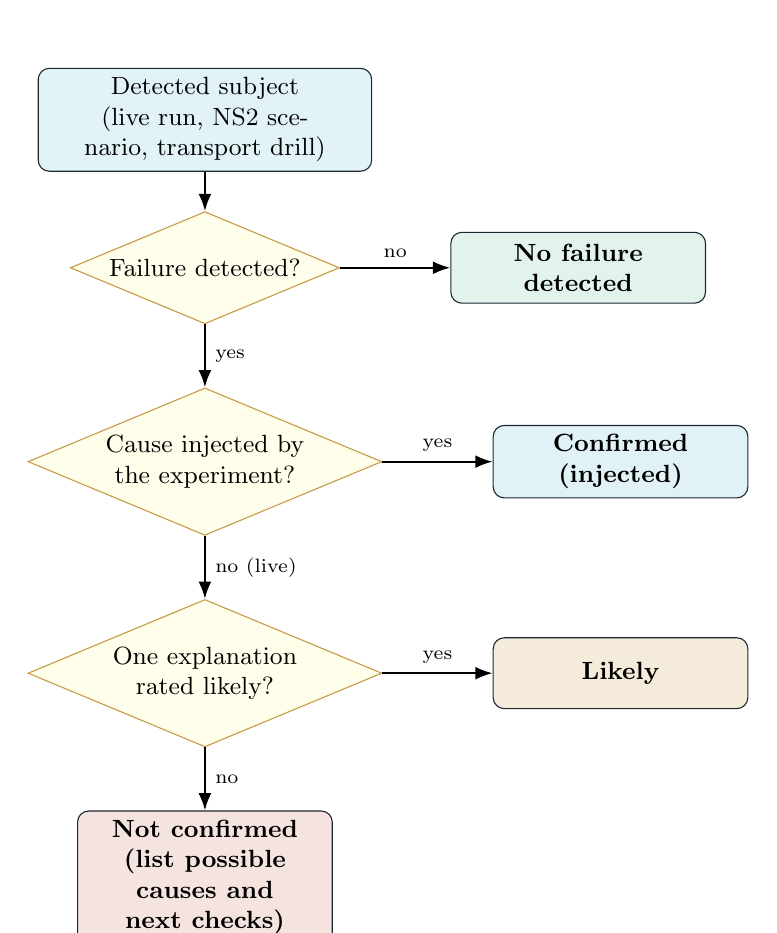
\begin{tikzpicture}[
  node distance=5mm,
  stage/.style={draw=RouteInk,rounded corners=4pt,align=center,text width=40mm,minimum height=9mm,fill=RoutePale,font=\small},
  decision/.style={diamond,draw=RouteAmber,aspect=2.4,align=center,fill=yellow!8,font=\small,inner sep=0.8pt,text width=27mm},
  status/.style={draw=RouteInk,rounded corners=4pt,align=center,text width=30mm,minimum height=9mm,font=\small\bfseries},
  arrow/.style={-{Latex[length=2.2mm]},thick}
]
\node[stage,fill=RouteCyan!14] (in) {Detected subject (live run, NS2 scenario, transport drill)};
\node[decision,below=of in] (fail) {Failure detected?};
\node[decision,below=8mm of fail] (inj) {Cause injected by the experiment?};
\node[decision,below=8mm of inj] (lik) {One explanation rated likely?};
\node[status,right=14mm of fail,fill=RouteGreen!15] (none) {No failure detected};
\node[status,right=14mm of inj,fill=RouteCyan!15] (conf) {Confirmed (injected)};
\node[status,right=14mm of lik,fill=RouteAmber!20] (likely) {Likely};
\node[status,below=8mm of lik,fill=RouteClay!18] (nc) {Not confirmed (list possible causes and next checks)};
\draw[arrow] (in) -- (fail);
\draw[arrow] (fail) -- node[above,font=\scriptsize]{no} (none);
\draw[arrow] (fail) -- node[right,font=\scriptsize]{yes} (inj);
\draw[arrow] (inj) -- node[above,font=\scriptsize]{yes} (conf);
\draw[arrow] (inj) -- node[right,font=\scriptsize]{no (live)} (lik);
\draw[arrow] (lik) -- node[above,font=\scriptsize]{yes} (likely);
\draw[arrow] (lik) -- node[right,font=\scriptsize]{no} (nc);
\end{tikzpicture}
\caption{Flowchart for assigning a cause status in the root-cause register}
\label{fig:causeflow}
\end{figure}

\subsection{NS2 Simulation Methodology}
The NS2 model in Figure~\ref{fig:topology} contains source node \texttt{n0}, destination node \texttt{n5}, access nodes \texttt{n1} and \texttt{n4}, and two core alternatives through \texttt{n2} and \texttt{n3}. The primary core links use 2 Mb/s, 10 ms delay and routing cost 1; the alternative links use 2 Mb/s, 15 ms and cost 3; access links use 10 Mb/s and 2 ms. Every queue is DropTail with a 20-packet limit. The monitored flow is a 1 Mb/s constant-bit-rate UDP stream of 1000-byte packets from \texttt{n0} to \texttt{n5}, active from 1 to 9 s. Four scenarios reuse the same topology and traffic: A, healthy baseline; B1, link \texttt{n1--n2} down from 3 to 6 s with distance-vector routing; B2, the same failure with static routing; and C, congestion from a second 1.5 Mb/s flow between 3 and 6 s. NS2 runs locally through a Docker image and on the hosted deployment through the Debian \texttt{ns2} package.

\begin{figure}[H]
\centering
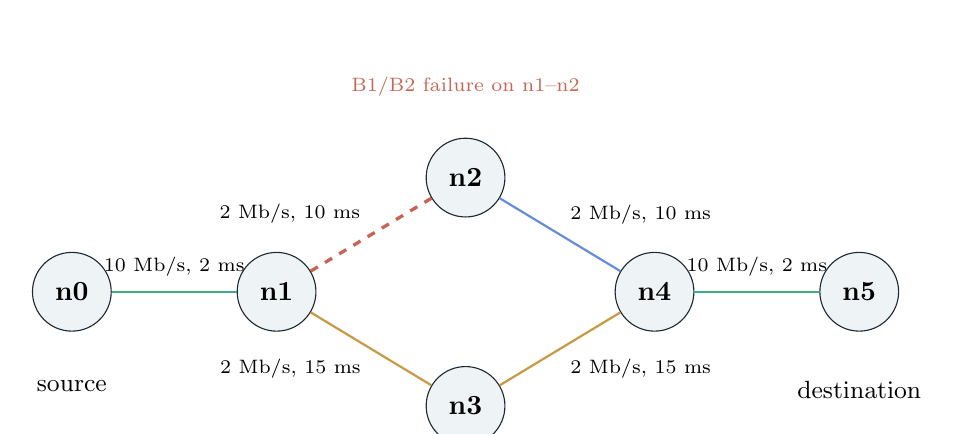
\begin{tikzpicture}[
  router/.style={circle,draw=RouteInk,fill=RoutePale,minimum size=10mm,font=\bfseries},
  primary/.style={thick,draw=RouteBlue},
  alternate/.style={thick,draw=RouteAmber},
  access/.style={thick,draw=RouteGreen},
  failed/.style={very thick,draw=RouteClay,dashed}
]
\node[router] (n0) at (0,0) {n0};
\node[router] (n1) at (2.6,0) {n1};
\node[router] (n2) at (5.0,1.45) {n2};
\node[router] (n3) at (5.0,-1.45) {n3};
\node[router] (n4) at (7.4,0) {n4};
\node[router] (n5) at (10.0,0) {n5};
\draw[access] (n0) -- node[above=2pt,font=\scriptsize]{10 Mb/s, 2 ms} (n1);
\draw[failed] (n1) -- node[above left,font=\scriptsize]{2 Mb/s, 10 ms} (n2);
\draw[primary] (n2) -- node[above right,font=\scriptsize]{2 Mb/s, 10 ms} (n4);
\draw[alternate] (n1) -- node[below left,font=\scriptsize]{2 Mb/s, 15 ms} (n3);
\draw[alternate] (n3) -- node[below right,font=\scriptsize]{2 Mb/s, 15 ms} (n4);
\draw[access] (n4) -- node[above=2pt,font=\scriptsize]{10 Mb/s, 2 ms} (n5);
\node[below=5mm of n0,font=\small]{source};
\node[below=5mm of n5,font=\small]{destination};
\node[above=4mm of n2,font=\scriptsize,text=RouteClay]{B1/B2 failure on n1--n2};
\end{tikzpicture}
\caption{Six-node NS2 topology with primary and alternative paths}
\label{fig:topology}
\end{figure}

Each trace line becomes an event, and NS2 packet identifiers prevent a packet forwarded by several routers from being counted more than once. For the set $S$ of monitored packets sent in a window, the set $R\subseteq S$ delivered, the set $D$ lost and the set $F$ still in flight when the simulation ends, the analyser computes loss, average one-way delay, jitter and throughput as
\begin{align}
L &= \frac{|D|}{|S| - |F|} \times 100\,\%, \label{eq:loss}\\
\bar d &= \frac{1}{|R|}\sum_{p\in R}\left(t^{\mathrm{recv}}_p - t^{\mathrm{send}}_p\right), \label{eq:delay}\\
J &= \frac{1}{|R|-1}\sum_{k=2}^{|R|}\left|d_k - d_{k-1}\right|, \label{eq:jitter}\\
T &= \frac{\sum_{p\in R} 8\,s_p}{t_{\mathrm{end}} - t_{\mathrm{start}}}, \label{eq:throughput}
\end{align}
where $d_k$ is the delay of the $k$-th delivered packet in send order and $s_p$ is the packet size in bytes. Loss and delay assign packets to a phase by send time; throughput uses receive time. Recovery after a failure at $t_{\mathrm{fail}}$ is quantified as the time until the first packet is delivered over the alternative path,
\begin{equation}
t_{\mathrm{rec}} = t^{\mathrm{recv}}_{\mathrm{first\,alt}} - t_{\mathrm{fail}},
\label{eq:recovery}
\end{equation}
and is reported only when the trace actually contains such a delivery. NS2 2.35 writes no drop line for packets discarded at a router whose route points to a down link, so those losses are inferred from each packet's last traced event and labelled as inferred.

\subsection{Transport and Security Methodology}
TCP uses length-prefixed frames with exact partial-read handling. Sequenced UDP datagrams expose gaps, duplicates, reordering and idle timeout without adding retransmission. TLS uses Python's \texttt{ssl} module \cite{python_ssl} with TLS 1.2 or later \cite{tls13}, mandatory certificate and host-name validation, and a locally generated lab PKI. The client and server SHA-256 digests \cite{sha} of every payload must match. Six drills inject a known transport fault (no listener, silent server, mid-transfer reset, skipped UDP sequence numbers, untrusted issuer, wrong host name), record the resulting error, and then repeat the operation under restored conditions to verify recovery.

% =============================================================================
\chapter{Implementation \& Testing}
% =============================================================================

\section{Experimental Setup}
\subsection{Hardware, Software and Tools}
The hardware, software, tools and configuration used to implement and test RouteResQ are listed in Table~\ref{tab:setup}.

\begin{table}[H]
\centering
\caption{Hardware and software environment}
\label{tab:setup}
\tighttable
\begin{tabularx}{\textwidth}{>{\bfseries\raggedright\arraybackslash}p{0.24\textwidth}X}
\toprule
Item & Configuration\\
\midrule
Development platform & Windows 11 computer with Python 3.13 for local diagnostics, loopback socket experiments and tests.\\
Deployment & Streamlit Community Cloud (Python 3.12, Debian Linux) at \nolinkurl{routeresq.streamlit.app}; public mode restricts probes.\\
Application framework & Streamlit multipage application with a workflow rail, Plotly charts and cached readers.\\
Simulation & NS2 2.35 in the Docker image \texttt{routeresq-ns2:2.35} locally and the Debian \texttt{ns2} package on the cloud host.\\
Networking tools & Windows \texttt{ping}, \texttt{tracert}, \texttt{route}, \texttt{ipconfig}; Linux \texttt{ping}, \texttt{traceroute}, \texttt{ip}.\\
Communication & Python TCP and UDP sockets, threaded local servers, length-prefixed framing, sequence-aware datagrams.\\
Security & Python \texttt{ssl}/OpenSSL, lab PKI generated with the \texttt{cryptography} package, TLS 1.2 minimum, SHA-256 digests.\\
Evidence storage & JSON, JSONL, CSV, Markdown, NS2 trace and event-log files under \texttt{results/} and \texttt{reports/}.\\
Testing & Pytest suite of 159 tests with markers \texttt{ns2}, \texttt{network} and \texttt{ui}; Streamlit AppTest for pages.\\
\bottomrule
\end{tabularx}
\end{table}

\subsection{Implementation and Configuration}
The interface follows the operational sequence Overview, Detect, Diagnose, Analyse impact, Observe recovery, Transport lab and Report, shown as a navigation rail in which each stage displays a live headline from stored results. A guided demonstration page executes the whole sequence and marks each stage as succeeded, partial or failed only after checking its stored evidence. Every page carries a source label such as live measurement, NS2 simulation or real sockets on loopback, and follows the same structure: a short explanation, key measurements, charts or tables, an interpretation, the method, and the artefacts consumed and produced.

The backend is independent of Streamlit. Diagnostics can be launched from the command line, simulation traces can be re-analysed without re-running NS2, communication experiments can use loopback or two laboratory computers, and reports such as the root-cause register (\texttt{python -m analysis.cause\_report}) are generated directly from stored results. Rule thresholds are kept in \texttt{config/thresholds.json} and authorised destinations in a separate policy file, so the analysis can be tuned without changing code.

\subsection{Testing Strategy}
Testing covers deterministic units and real integrations. Captured command fixtures from Windows and Linux verify parser behaviour for reachable hosts, DNS errors, timeouts, partial and complete loss, sub-millisecond RTTs, unreachable responses, truncated output and different traceroute formats. Mocked measurements drive each root-cause rule and contradiction. Real sockets verify framing, TCP and UDP transfers, TLS identity and integrity, and recovery after injected failures. NS2 integration tests check the expected behaviour of all four scenarios when the simulator is available, and Streamlit AppTest exercises every page and the guided workflow. All 159 tests pass on the development machine.

\section{Results (Test Cases / Screenshots / Output)}
\subsection{Test Cases}
Representative validation cases and their verified outcomes are listed in Table~\ref{tab:testcases}. TC1 to TC3 exercise the live pipeline on destinations reserved for testing \cite{rfc5737,rfc6761}; TC4 to TC7 use the NS2 scenarios; TC8 to TC11 use real sockets and the cause register.

\begin{table}[H]
\centering
\caption{Representative test cases and verified outcomes}
\label{tab:testcases}
\tighttable
\begin{tabularx}{\textwidth}{p{0.07\textwidth}>{\raggedright\arraybackslash}p{0.27\textwidth}>{\raggedright\arraybackslash}X}
\toprule
\textbf{ID} & \textbf{Test} & \textbf{Verified outcome}\\
\midrule
TC1 & Reachable loopback destination & DNS resolves, 4/4 echo replies, 0\% loss by Eq.~\eqref{eq:liveloss}, one-hop path, \emph{Healthy / Reachable}.\\
TC2 & Reserved invalid name (\nolinkurl{nonexistent.invalid}) & DNS failure recorded; no connection attempted; cause \emph{Likely}: name does not exist.\\
TC3 & Documentation address timeout (\texttt{192.0.2.1}) & Unreachable, 100\% loss; cause \emph{Not confirmed} with three possible causes and next checks.\\
TC4 & NS2 healthy baseline & 1001/1001 packets delivered with 33.6 ms average delay.\\
TC5 & DV link failure & Alternative path observed; 999/1001 delivered; two route changes recorded.\\
TC6 & Static link failure & No delivery during the event; service resumes after restoration.\\
TC7 & Congestion & Queue reaches 20 packets; delay and loss rise during excess offered load.\\
TC8 & TCP and UDP comparison & Real sockets complete; TCP integrity matches and UDP sequence gaps are detectable.\\
TC9 & TLS secure transfer & Certificate chain, host name, protocol, cipher and SHA-256 digest verified.\\
TC10 & Failure drills & Refusal, timeout, reset, missing datagrams and certificate errors detected; recovery checked.\\
TC11 & Root-cause register & 11 of 13 subjects carry a stated cause; 2 healthy subjects are marked \emph{No failure detected}.\\
\bottomrule
\end{tabularx}
\end{table}

\subsection{Command Centre}
The overview page in Figure~\ref{fig:overview} is the entry point of the application. It shows the brand bar with the detected NS2 and tool status, the workflow rail, and key results read from stored evidence, such as the distance-vector reroute time of 43.6 ms and the static-route outage of 3.02 s.

\begin{figure}[htbp]
\centering
\includegraphics[width=0.86\textwidth]{\asset{overview.jpg}}
\caption{Command centre with workflow rail and stored key results}
\label{fig:overview}
\end{figure}

\subsection{Live Diagnostic Results}
A controlled run against \texttt{localhost} verified the live measurement pipeline without probing an external system. The platform resolved both loopback addresses, received four of four echo replies, computed 0\% loss with Eq.~\eqref{eq:liveloss}, and observed a one-hop path. The conclusion was \emph{Healthy / Reachable}. Figure~\ref{fig:diagnostics} shows the configuration, completion state, conclusion and KPI values together.

\begin{figure}[htbp]
\centering
\includegraphics[width=0.74\textwidth]{\asset{diagnostics.jpg}}
\caption{Live loopback diagnostic with measured healthy result}
\label{fig:diagnostics}
\end{figure}

The root-cause page evaluated all rules for the same run. Only the healthy-state rule fired, so no problem finding or candidate cause was generated. The evidence ladder in Figure~\ref{fig:rootcause} keeps symptoms, measurements, explanations and limitations separate; even a healthy run states that ICMP-based tools see only the devices that choose to answer.

\begin{figure}[htbp]
\centering
\includegraphics[width=0.74\textwidth]{\asset{root_cause.jpg}}
\caption{Deterministic diagnostic reasoning and complete rule trace}
\label{fig:rootcause}
\end{figure}

\subsection{Root-Cause Register}
The root-cause register is the output that answers the project's main question: \emph{what caused each failure, and how sure are we?} It joins the latest live run per destination, the four NS2 scenarios and the transport drills, and applies the decision procedure of Figure~\ref{fig:causeflow}. Table~\ref{tab:register} summarises the generated register, and Figure~\ref{fig:reports} shows the report page on which it is displayed.

\begin{longtable}{>{\raggedright\arraybackslash}p{0.17\textwidth}>{\raggedright\arraybackslash}p{0.20\textwidth}>{\raggedright\arraybackslash}p{0.15\textwidth}>{\raggedright\arraybackslash}p{0.36\textwidth}}
\caption{Root-cause register generated from stored results}\label{tab:register}\\
\toprule
\textbf{Source} & \textbf{Subject / failure} & \textbf{Status} & \textbf{Stated root cause}\\
\midrule
\endfirsthead
\toprule
\textbf{Source} & \textbf{Subject / failure} & \textbf{Status} & \textbf{Stated root cause}\\
\midrule
\endhead
Live diagnostics & \nolinkurl{nonexistent.invalid}: DNS resolution failure & Likely & The name does not exist in DNS or is misspelt; the gateway answered, so the local network works.\\
Live diagnostics & \texttt{192.0.2.1}: unreachable, packet loss & Not confirmed & Host down, path beyond the last responding hop (TTL 2) inaccessible, or ICMP filtered; a TCP check would separate them.\\
Live diagnostics & \texttt{8.8.8.8}: none & No failure detected & No failure to explain.\\
NS2 simulation & B1: link failure \texttt{n1--n2} & Confirmed (injected) & Link disabled by \texttt{rtmodel-at 3.0 down} and restored at 6.0 s.\\
NS2 simulation & B2: link failure \texttt{n1--n2} & Confirmed (injected) & Same link failure; static routing is the second controlled condition.\\
NS2 simulation & C: congestion on \texttt{n1--n2} & Confirmed (injected) & Competing 1.5 Mb/s flow from 3 to 6 s; offered load 2.5 Mb/s on a 2 Mb/s link.\\
NS2 simulation & A: none (control) & No failure detected & No fault introduced.\\
Transport drill & Connection timeout & Confirmed (injected) & Server accepts the connection but never replies; read timeout 1.5 s.\\
Transport drill & Interrupted TCP transfer & Confirmed (injected) & Server resets after about 300,000 of 2,000,000 bytes.\\
Transport drill & TLS host-name mismatch & Confirmed (injected) & Certificate issued for \texttt{wrong-host.example}, client expects \texttt{localhost}.\\
Transport drill & TLS untrusted issuer & Confirmed (injected) & Certificate signed by a CA the client does not trust.\\
Transport drill & Missing UDP datagrams & Confirmed (injected) & Sender skipped sequence numbers 50--54, 120 and 199.\\
Transport drill & Server unavailable & Confirmed (injected) & No process listening on the selected loopback port.\\
\bottomrule
\end{longtable}

Eleven failures were explained out of thirteen subjects. The two live failures show the certainty model at work: a DNS failure with a working gateway has exactly one consistent explanation and is reported as \emph{Likely}, whereas an unreachable documentation address is consistent with three explanations and is honestly reported as \emph{Not confirmed}, together with the checks that would separate them.

\begin{figure}[htbp]
\centering
\includegraphics[width=0.86\textwidth]{\asset{reports.jpg}}
\caption{Report page with the root-cause report and experiment history}
\label{fig:reports}
\end{figure}

\subsection{NS2 Results}
Table~\ref{tab:ns2results} compares delivery, loss (Eq.~\eqref{eq:loss}), average delay (Eq.~\eqref{eq:delay}), throughput (Eq.~\eqref{eq:throughput}), route changes and recovery across the four stored scenarios.

\begin{table}[H]
\centering
\caption{Comparison of stored NS2 experiment results}
\label{tab:ns2results}
\begin{tabularx}{\textwidth}{>{\bfseries}p{0.17\textwidth}rrrrr>{\raggedright\arraybackslash}X}
\toprule
Scenario & Delivered & Loss & Avg. delay & Throughput & Route & Recovery\\
 &  & (\%) & (ms) & (kb/s) & changes & \\
\midrule
Healthy A & 1001/1001 & 0.00 & 33.60 & 996.81 & 0 & Not applicable\\
DV failure B1 & 999/1001 & 0.20 & 37.36 & 994.82 & 2 & Rerouted over alternative path\\
Static failure B2 & 624/1001 & 37.66 & 33.60 & 621.39 & 0 & Resumed after link restoration\\
Congestion C & 884/1001 & 11.69 & 54.55 & 880.30 & 0 & Delay and loss returned to baseline\\
\bottomrule
\end{tabularx}
\end{table}

In B1, link \texttt{n1--n2} was disabled from 3 to 6 s while distance-vector routing was active. Forwarding changed from \texttt{0--1--2--4--5} to \texttt{0--1--3--4--5}. Only two packets were lost, all 375 packets sent during the down interval were delivered, and by Eq.~\eqref{eq:recovery} the first delivery on the alternative path arrived $t_{\mathrm{rec}} = 43.6$ ms after the failure. Average delay rose because the alternative route uses two 15 ms links.

In B2, the identical link failure was combined with static routing. Node \texttt{n1} continued to forward toward the failed link, so none of the 375 packets sent during the event reached the destination. The destination experienced a 3.024 s delivery gap and service returned only when the link was restored. In C, the monitored 1 Mb/s flow and a competing 1.5 Mb/s flow offered 2.5 Mb/s to a 2 Mb/s core link. The queue reached its 20-packet limit, during-phase delay rose to 102.75 ms, and queue overflow caused loss. Figure~\ref{fig:simcharts} shows the B1 throughput and path-dependent delay reconstructed from the trace.

\begin{figure}[htbp]
\centering
\includegraphics[width=0.74\textwidth]{\asset{simulation_charts.jpg}}
\caption{B1 throughput and path-dependent delay reconstructed from the NS2 trace}
\label{fig:simcharts}
\end{figure}

\subsection{Failure and Recovery Results}
Recovery is claimed only when the trace shows an observable event. For B1 the platform records the configured link-down event, the traced link-down event, the first dropped packet, the burst of routing updates, the first packet on the alternative route, the later link-up event and the switch back to the primary path. Figure~\ref{fig:recovery} presents the recovery verdict and the selected scenario without hiding the experimental cause.

\begin{figure}[htbp]
\centering
\includegraphics[width=0.74\textwidth]{\asset{recovery.jpg}}
\caption{Trace-backed distance-vector recovery verdict}
\label{fig:recovery}
\end{figure}

The three failure experiments illustrate different recovery mechanisms, compared in Table~\ref{tab:recovery}. Distance-vector routing maintained delivery by changing path; static routing waited for the failed link to return; congestion recovered when offered load fell and the queue drained. These outcomes cannot be reduced to one generic status because they represent rerouting, restoration and performance recovery respectively.

\begin{table}[H]
\centering
\caption{Recovery evidence by scenario}
\label{tab:recovery}
\tighttable
\begin{tabularx}{\textwidth}{>{\bfseries\raggedright\arraybackslash}p{0.16\textwidth}>{\raggedright\arraybackslash}p{0.22\textwidth}>{\raggedright\arraybackslash}p{0.22\textwidth}>{\raggedright\arraybackslash}X}
\toprule
Scenario & Failure mechanism & Observation & Recovery evidence\\
\midrule
B1 DV & Primary link down & Path changes twice & First alternative-path delivery 43.6 ms after failure; after-phase throughput 101.9\% of before.\\
B2 Static & Primary link down & 375 event-window packets not delivered & Delivery returns after the trace records link restoration; 3.024 s gap.\\
C Congestion & Offered load exceeds capacity & Queue fills and DropTail discards arrivals & Delay and loss return near baseline after the competing flow stops and the queue drains.\\
\bottomrule
\end{tabularx}
\end{table}

\subsection{TCP, UDP and TLS Results}
The communication report contains three 1,000,000-byte TCP trials and three UDP trials on loopback. Every TCP trial delivered all bytes and produced a matching SHA-256 digest. All UDP datagrams also arrived in these particular trials, but the platform does not treat that as a UDP guarantee. The measured mean throughput was 3067.1 Mb/s for TCP and 840.4 Mb/s for UDP on this host; these figures describe loopback and are not a general ranking of the protocols. Figure~\ref{fig:tcp} records the framed TCP exchange.

\begin{figure}[htbp]
\centering
\includegraphics[width=0.74\textwidth]{\asset{transport_tcp.jpg}}
\caption{Real framed TCP message exchange on loopback}
\label{fig:tcp}
\end{figure}

Figure~\ref{fig:tls} shows a fresh 262,144-byte payload sent over TLS. The backend verified the TCP connection, the TLS handshake, the certificate chain to the lab CA, the host-name match for \texttt{localhost}, the framed data transfer, equal client and server SHA-256 digests, and an orderly close. The run negotiated TLS 1.3 with an AES-256-GCM cipher suite.

\begin{figure}[htbp]
\centering
\includegraphics[width=0.74\textwidth]{\asset{transport_tls.jpg}}
\caption{Verified TLS transfer with certificate and SHA-256 checks}
\label{fig:tls}
\end{figure}

\subsection{Controlled Failure Demonstrations}
Six controlled drills connect an injected cause to an observed protocol error and then to an explicit restoration check, as listed in Table~\ref{tab:failures}. This gives each error a known ground truth without claiming that the same message proves the same cause on a live network.

\begin{longtable}{>{\raggedright\arraybackslash}p{0.19\textwidth}>{\raggedright\arraybackslash}p{0.28\textwidth}>{\raggedright\arraybackslash}p{0.24\textwidth}>{\raggedright\arraybackslash}p{0.18\textwidth}}
\caption{Transport failure drills and recovery checks}\label{tab:failures}\\
\toprule
\textbf{Failure} & \textbf{Injected cause} & \textbf{Observed evidence} & \textbf{Recovery}\\
\midrule
\endfirsthead
\toprule
\textbf{Failure} & \textbf{Injected cause} & \textbf{Observed evidence} & \textbf{Recovery}\\
\midrule
\endhead
Server unavailable & No process listening on the selected loopback port & Connection refused; no application data sent & Start server; message acknowledged\\
Connection timeout & Server accepts TCP but never replies & Client read timeout after 1.5 s & Replace with responsive server\\
Interrupted transfer & Server sends reset after part of a 2,000,000-byte payload & Connection reset; no final acknowledgement & Restart and resend; digest matches\\
Missing UDP datagrams & Sequence numbers 50--54, 120 and 199 deliberately skipped & Receiver reports exact missing ranges and idle timeout & Repeat without skips; 200/200 received\\
Untrusted certificate & Server certificate signed by an untrusted CA & TLS certificate verification error & Switch to certificate signed by lab CA\\
Host-name mismatch & Lab-CA certificate issued for a different host & Host-name verification error & Present valid \texttt{localhost} certificate\\
\bottomrule
\end{longtable}

\subsection{Guided Demonstration and Generated Reports}
The guided demonstration runs a live diagnostic, the rule engine, the NS2 analysis, the recovery check, the transport experiments and report generation in order. A stage is marked as succeeded only when fresh evidence for it is found on disk; otherwise it is shown as partial, failed or not started, with the reason. The report page reads directly from stored results and lists the generated Markdown reports (healthy baseline, both link-failure scenarios, congestion, scenario comparison, live diagnostics, communication and the root-cause report), the diagnostic history, NS2 runs, communication results and raw evidence files, all of which can be downloaded. Every summary therefore remains traceable to its originating artefact.

% =============================================================================
\chapter{Conclusion \& Future Scope}
% =============================================================================

\section{Summary of Work and Achievements}
RouteResQ integrates live network diagnostics, deterministic root-cause reasoning, NS2 failure analysis, recovery observation, real TCP and UDP communication, TLS identity validation, payload integrity, controlled failure drills and evidence-driven reporting in one deployed application. It answers not only whether communication succeeded, but what failed, what caused it, how certain that cause is, which rule or trace event supports it, what alternatives remain, and what cannot be concluded. The root-cause register states a cause for 11 of the 13 recorded subjects, the NS2 experiments quantify rerouting in 43.6 ms against a 3.024 s outage under static routing, and the transport drills show six different failures and their recovery.

The strongest achievement is the separation of evidence environments. A live network result is never assigned a simulated cause; a trace-backed injected cause is labelled \emph{Confirmed (injected)} because the scenario configuration and the trace agree; and loopback transport results are reported as host-specific.

Object-oriented programming contributes directly to solving the problem:
\begin{sloppypar}
\begin{itemize}
  \item \textbf{Encapsulation and composition.} Each measurement is a data class (\texttt{DNSResult}, \texttt{PingResult}, \texttt{TracerouteResult}, \texttt{TCPCheckResult}) composed into one \texttt{DiagnosticRun}; the analysis output is likewise an \texttt{AnalysisReport} composed of \texttt{Finding}, \texttt{Explanation} and \texttt{RuleTrace} objects. Evidence therefore travels as one consistent, serialisable object from measurement to report.
  \item \textbf{Abstraction and polymorphism.} The \texttt{CommandRunner} protocol hides how commands are executed. \texttt{SubprocessRunner} runs real allow-listed tools, while the tests pass a fake runner that replays captured output, so the same rule engine is verified on Windows and Linux output without network access.
  \item \textbf{Inheritance.} Domain errors such as \texttt{TargetNotAllowed}, \texttt{ScenarioError}, \texttt{NS2UnavailableError}, \texttt{ConnectionClosed} and \texttt{ProtocolError} specialise built-in exception classes, so callers can handle a category of failure precisely.
  \item \textbf{Validation inside objects.} A \texttt{Scenario} validates its identifier, category and parameters in its constructor, and \texttt{TCPTransferServer} is a context manager that always releases its socket, preventing invalid experiments and leaked resources.
  \item \textbf{Single responsibility.} Parsers, rules, scenario execution, trace analysis, socket transfer, PKI and reporting are separate classes and modules, which made 159 targeted tests possible and lets the interface consume stored results instead of duplicating calculations.
\end{itemize}
\end{sloppypar}

\section{Impact on Society, Environmental Sustainability, Ethical Issues and Compliance}
\noindent\textbf{Impact on society.} The platform gives students and administrators a repeatable path from command output to a justified explanation. Its reports teach precise language about certainty and make contradictory evidence visible, which reduces wrong diagnoses and the wasted repair effort that follows them.

\noindent\textbf{Environmental sustainability.} Simulation replaces dedicated networking hardware for routing and congestion experiments, and socket experiments run on existing computers. Faster fault isolation also reduces repeated testing and unnecessary traffic.

\noindent\textbf{Ethical issues and compliance.} Active probes are restricted to allow-listed, loopback, private or explicitly permitted destinations, and the public deployment restricts them further. Input is validated and commands are never executed through a shell. RouteResQ does not capture third-party traffic or store personal content. TLS relies on established libraries and a clearly labelled local lab PKI rather than custom cryptography, and every result is labelled as live, simulated or loopback so that no claim overstates its evidence.
\section{Limitations of the Work and Future Scope}
\noindent\textbf{Limitations.} Live accuracy depends on whether devices answer ICMP and path probes, and four ping samples give only coarse loss resolution. Live causes can be \emph{Likely} or \emph{Not confirmed} but never confirmed, because the true cause of a live failure is not known to the tool. The NS2 distance-vector model reacts faster than many real routing protocols, and its CBR/UDP congestion case does not model TCP congestion control. Loopback throughput excludes propagation delay and realistic path loss; the lab PKI is not a production authority; and RouteResQ explains recovery rather than repairing arbitrary live networks.

\noindent\textbf{Future scope.} Future work can add larger topologies, link-state routing with configurable convergence timers, two-computer laboratory experiments, trend analysis of repeated live runs, DNS and MTU drills, controlled bandwidth limits, and signed experiment manifests. Each extension should keep every conclusion linked to its evidence.

% =============================================================================
\clearpage
\renewcommand{\bibname}{References}
\addcontentsline{toc}{chapter}{References}
\begin{thebibliography}{99}
\bibitem{ns2book} T. Issariyakul and E. Hossain, \emph{Introduction to Network Simulator NS2}, 2nd ed. New York, NY, USA: Springer, 2012.
\bibitem{tcp} W. Eddy, Ed., ``Transmission Control Protocol (TCP),'' IETF RFC 9293, Aug. 2022. [Online]. Available: \url{https://www.rfc-editor.org/rfc/rfc9293}
\bibitem{udp} J. Postel, ``User Datagram Protocol,'' IETF RFC 768, Aug. 1980. [Online]. Available: \url{https://www.rfc-editor.org/rfc/rfc768}
\bibitem{tls13} E. Rescorla, ``The Transport Layer Security (TLS) Protocol Version 1.3,'' IETF RFC 8446, Aug. 2018. [Online]. Available: \url{https://www.rfc-editor.org/rfc/rfc8446}
\bibitem{sha} National Institute of Standards and Technology, ``Secure Hash Standard (SHS),'' FIPS PUB 180-4, Aug. 2015. [Online]. Available: \url{https://doi.org/10.6028/NIST.FIPS.180-4}
\bibitem{python_socket} Python Software Foundation, ``socket --- Low-level networking interface,'' Python 3 documentation. [Online]. Available: \url{https://docs.python.org/3/library/socket.html}
\bibitem{python_ssl} Python Software Foundation, ``ssl --- TLS/SSL wrapper for socket objects,'' Python 3 documentation. [Online]. Available: \url{https://docs.python.org/3/library/ssl.html}
\bibitem{streamlit} Streamlit Inc., ``Streamlit documentation.'' [Online]. Available: \url{https://docs.streamlit.io/}
\bibitem{rfc5737} J. Arkko, M. Cotton, and L. Vegoda, ``IPv4 Address Blocks Reserved for Documentation,'' IETF RFC 5737, Jan. 2010.
\bibitem{rfc6761} S. Cheshire and M. Krochmal, ``Special-Use Domain Names,'' IETF RFC 6761, Feb. 2013.
\bibitem{repo} S. Grover, A. Sharma, P. Goel, and A. S. Kulashri, ``RouteResQ: source code and experiment artefacts,'' GitHub repository, 2026. [Online]. Available: \url{https://github.com/SaiGrover/RouteResQ}
\end{thebibliography}

% =============================================================================
\clearpage
\chapter*{Appendix}
\addcontentsline{toc}{chapter}{Appendix}
\setcounter{table}{0}
\renewcommand{\thetable}{A.\arabic{table}}
\section*{Team Roles and Contributions}
The source code, stored results and this report are available in the project repository \cite{repo}. Table~\ref{tab:team} records the primary contribution of each team member.

\begin{table}[H]
\centering
\caption{Team roles and primary contributions}
\label{tab:team}
\tighttable
\begin{tabularx}{\textwidth}{>{\bfseries\raggedright\arraybackslash}p{0.38\textwidth}X}
\toprule
Student & Primary contribution\\
\midrule
Saanvi Grover (2408030010) & Live diagnostics integration, Streamlit workflow and deployment, report consolidation.\\
Aditya Sharma (2408030019) & NS2 scenarios, routing and recovery analysis, metric verification.\\
Prankit Goel (2408030011) & TCP/UDP experiments, TLS integration and integrity verification.\\
Aaradhya Shankar Kulashri (2408030026) & Test cases, security review, report validation and documentation.\\
\bottomrule
\end{tabularx}
\end{table}

\end{document}
